\section{Auswertung}
\label{sec:Auswertung}
\subsection{Messdaten}
\label{subsec:messdaten}
Die bei dem Versuch aufgenommenen Messdaten sind in den Tabellen \ref{tab:mess1} und \ref{tab:mess2}
dargestellt.
\begin{table}[H]
    \centering
        \caption{Messdaten 1. Quelle:\cite{AP02}}
        \label{tab:mess1}
        \sisetup{table-format=3.2}
        \begin{tabular}{c c @{${}\pm{}$} c}
          \toprule
          {$U [\si{V}]$} & \multicolumn{2}{c}{$N [\si{\per\second}]$} \\
          \midrule
          320 &  161.20 &  12.70\\
          330 &  161.48 &  12.71\\
          340 &  159.67 &  12.64\\
          350 &  163.95 &  12.80\\
          360 &  164.77 &  12.84\\
          370 &  167.35 &  12.94\\
          380 &  166.60 &  12.91\\
          390 &  165.72 &  12.87\\
          400 &  166.58 &  12.91\\
          410 &  166.33 &  12.90\\
          420 &  166.43 &  12.90\\
          430 &  166.00 &  12.88\\
          440 &  170.32 &  13.05\\
          450 &  171.07 &  13.08\\
          460 &  169.57 &  13.02\\
          470 &  167.25 &  12.93\\
          480 &  172.50 &  13.13\\
          490 &  171.50 &  13.10\\
          500 &  169.18 &  13.01\\
          510 &  168.50 &  12.98\\
          520 &  170.92 &  13.07\\
          530 &  169.18 &  13.01\\
          540 &  172.52 &  13.13\\
          550 &  169.73 &  13.03\\
          560 &  168.95 &  13.00\\
          570 &  169.77 &  13.03\\
          580 &  169.52 &  13.02\\
          590 &  169.52 &  13.02\\
          600 &  170.88 &  13.07\\
          610 &  172.80 &  13.15\\
          620 &  172.75 &  13.14\\
          630 &  170.40 &  13.05\\
          640 &  172.30 &  13.13\\
          650 &  174.88 &  13.22\\
          660 &  174.45 &  13.21\\
          670 &  177.33 &  13.32\\
          680 &  182.32 &  13.50\\
          690 &  185.98 &  13.64\\
          700 &  192.45 &  13.87\\
          \bottomrule
        \end{tabular}
      \end{table}

\begin{table}[H]
  \centering
      \caption{Messdaten 2. Quelle:\cite{AP02}}
      \label{tab:mess2}
      \sisetup{table-format=3.2}
      \begin{tabular}{c c @{${}\pm{}$} c c @{${}\pm{}$} c}
        \toprule
        {$U [\si{V}]$} & 
        \multicolumn{2}{c}{$N [\si{\per\second}]$}  & 
        \multicolumn{2}{c}{$I [\si{\micro\ampere}]$}\\
        \midrule
        350 & 163.95 & 12.80 & 0.30 & 0.05\\
        400 & 166.58 & 12.91 & 0.40 & 0.05\\
        450 & 171.07 & 13.08 & 0.70 & 0.05\\
        500 & 169.18 & 13.01 & 0.80 & 0.05\\
        550 & 169.73 & 13.03 & 1.00 & 0.05\\
        600 & 170.88 & 13.07 & 1.30 & 0.05\\
        650 & 174.88 & 13.22 & 1.40 & 0.05\\
        700 & 192.45 & 13.87 & 1.80 & 0.05\\
        \bottomrule
      \end{tabular}
    \end{table}
    
\subsection{Die Zählrohr-Charakteristik}
\label{subsec:Charakteristik}
Da die Zählrate Poission verteilt ist, ist die Messunsicherheit gegeben durch 
\begin{equation}
    \Delta N=\sqrt{N}. \label{eqn:Wurzel}
\end{equation}
In Abbildung \ref{fig:Kennlinie} ist die Zählrate $N$ gegen die Spannung $U$ aufgetragen. Die Fehlerbalken
ergeben sich dabei aus Gleichung \ref{eqn:Wurzel}.
\begin{figure}[H]
    \centering
    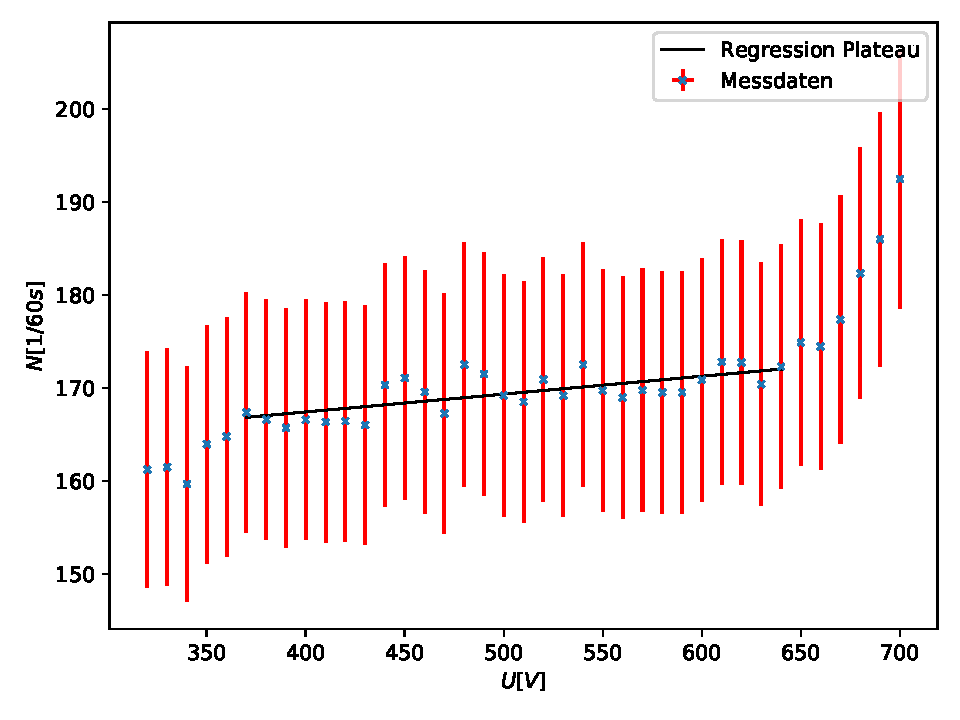
\includegraphics[scale=0.8]{auswertung/plot1.pdf}
    \caption{Kennlinie mit linearer Regression an dem Plateau}
    \label{fig:Kennlinie}
  \end{figure}
  \noindent Durch Ablesen kann nun das Plateau-Intervall auf $I_{P}=[\SI{370}{\volt}, \SI{640}{\volt}]$ geschätzt werden.
  Die Länge die Plateaus beträgt somit $l_{P}=\SI{270}{\volt}$. Für das Intervall 
  wurde von \textit{python} eine Regression durchgeführt. Diese hat eine Funktionsgleichung der Form
  \begin{equation}
      y=a\cdot x+b \label{eqn:gerade}
  \end{equation} 
  mit
  \begin{align*}
    a &= \SI{0.0192 \pm 0.0037}{\per\volt\per\second}\\
    b &= \SI{159.74 \pm 1.9065}{\per\second}.
  \end{align*}
  Die Unsicherheiten wurden dabei von  \textit{nummeric python} berechnet.
  Die Plateau-Steigung entspricht demnach
  \begin{equation*}
    a = \SI{1.92 \pm 0.37}{\percent\per\volt\per\second}.
  \end{equation*}

\subsection{Der zeitliche Abstand zwischen Primär- und Nachentladungsimpulsen}
\label{subsec:abstand}
Der zeitliche Abstand zwischen Primär- und Nachentladungsimpulsen erfolgt über Ablesen von einem
Oszilloskop. Das dafür verwendete Bild ist dabei in Abbildung \ref{fig:Osz} dargestellt. Die Zeitachse
am Oszilloskop ist $\SI{100}{\micro\second}/\text{DIV}$.
\begin{figure}[H]
    \centering
    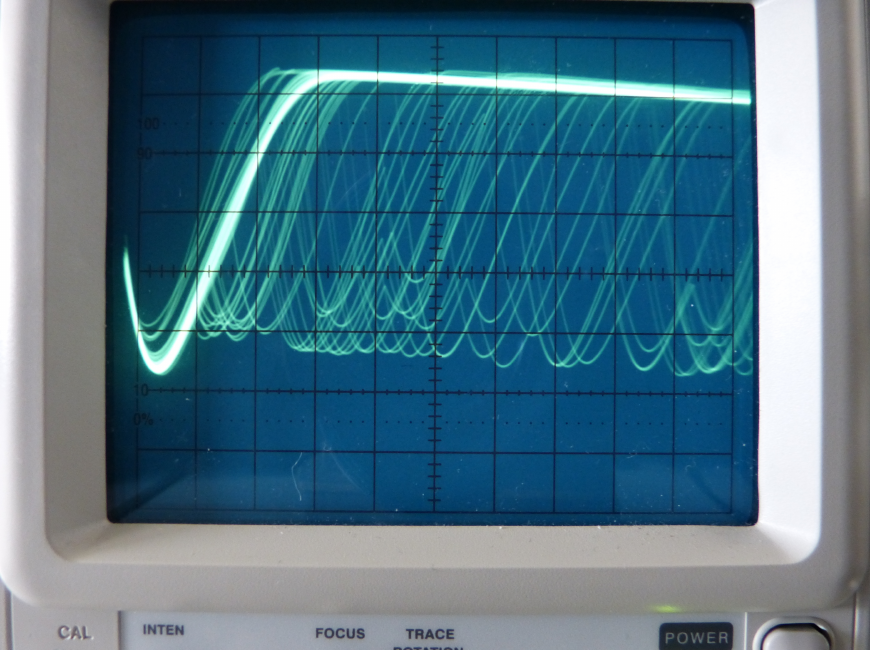
\includegraphics[scale=0.5]{content/Osz.png}
    \caption{Spannungs-Zeit-Messung mittels Oszilloskop. Quelle:\cite{AP02}}
    \label{fig:Osz}
  \end{figure}
Durch dieses Vorgehen ergibt sich
\begin{align*}
    t_{Abstand}&=\SI{170}{\micro\second}-\SI{120}{\micro\second}\\
               &=\SI{50}{\micro\second}.
\end{align*}

\subsection{Die Totzeit}
\label{subsec:totzeit}
Die Totzeit kann auf zwei verschiedenen Wegen ermittelt werden. Zum einen kann diese von einem Oszilloskop
abgelesen und zum andere durch die Zwei-Quellen-Methode bestimmt werden. 
In diesem Unterkapitel wird die Totzeit durch beide Methoden ermittelt und die Abweichung der Werte 
berechnet. 
\subsubsection*{Abesen vom Oszilloskop}
        Auch die Totzeit kann durch Ablesen von Abbildung \ref{fig:Osz} bestimmt werden. Das liefert
        $t_{tot-Osz}=\SI{160}{\micro\second}$.
\subsubsection*{Berechnung mit Zwei-Quellen-Methode}
        Bei der Zwei-Quellen-Methode wurden die Messwerte
        \begin{align*}
            N_1 &= \SI{800.34}{\per\per\second}\\ %Müssen hier Unsicherheiten hin?
            N_{1+2} &= \SI{637.65}{\per\per\second}\\
            N_2 &= \SI{1320.66}{\per\per\second}
        \end{align*}
        aufgenommenen \cite{AP02}. Nun wird durch 
        \begin{equation*}
            t_{tot}\approx \frac{N_1+N_2-N_{1+2}}{2N_1N_2}
        \end{equation*}
        die Totzeit berechnet. Einsetzen ergibt $t_{tot-2Q}=\SI{114.96 \pm 47.27}{\micro\second}$.
\subsubsection*{Prozentuale Abweichung}
Die prozentuale Abweichung der beiden Werte kann durch 
\begin{equation}
    p_{abw}=\frac{t_{tot-Q}-t_{tot-Osz}}{t_{tot-2Q}}\cdot 100
\end{equation}
berechnet werden. Durch Einsetzen ergibt sich $p_{abw}=\num{-39.18}\%$.

\subsection{Freigesetzte Ladung pro Teilchen}
\label{subsec:Ladung}
Die freigesetzte Ladung pro Teilchen lässt sich durch
\begin{equation}
    Q=\frac{\bar{I}}{N} \label{eqn:Q}
\end{equation}
berechnen. $\bar{I}$ ist dabei das arithmetische Mittel der Werte von $I$, die aus Tabelle \ref{tab:mess2}
zu entnehmen sind. Das arithmetische Mittel ist dabei durch 
\begin{equation*}
    \bar{x}_\text{k} = \frac{1}{N} \sum_{k = 1}^{N} x_\text{k}
\end{equation*} 
gegeben. Durch Einsetzen ergibt sich für den Mittelwert $\bar{I}=\SI{0.96 \pm 0.18}{\micro\ampere}$.
Die mit Gleichung \ref{eqn:Q} berechneten Werte für $Q$ sind in Tabelle \ref{tab:ladungproteilchen} 
aufgelistet.
\begin{table}[H]
    \centering
    \caption{Die freigesetzte Ladungen pro Teilchen}
    \label{tab:ladungproteilchen}
    \begin{tabular}{c c @{${}\pm{}$} c c @{${}\pm{}$} c}
        \toprule
        $U \; [\si{\volt}]$ & 
        \multicolumn{2}{c} {$N \; [\si{\per\second}]$}   & 
        \multicolumn{2}{c} {$Q \; [\si{\giga}\symup{e_0}]$} \\ 
        \midrule
        350 & 163.95 & 12.80 & 36.64 & 7.50\\
        400 & 166.58 & 12.91 & 36.06 & 7.38\\
        450 & 171.07 & 13.08 & 35.12 & 7.17\\
        500 & 169.18 & 13.01 & 35.51 & 7.25\\
        550 & 169.73 & 13.03 & 35.39 & 7.23\\
        600 & 170.88 & 13.07 & 35.16 & 7.18\\
        650 & 174.88 & 13.22 & 34.35 & 7.00\\
        700 & 192.45 & 13.87 & 31.22 & 6.32\\    
        \bottomrule
    \end{tabular}
\end{table}

\noindent Die Anzah der freigesetzten Ladungen pro Teilchen wird durch
\begin{equation*}
    Z=\frac{I}{\symup{e_0}N},
\end{equation*}
berechnet, wobei $\symup{e_0}$ die Elementarladung ist.
\begin{table}[H]
    \centering
    \caption{Die Zahl der freigesetzten Ladungen pro Teilchen}
    \label{tab:zahlproteilchen}
    \begin{tabular}{c c @{${}\pm{}$} c c @{${}\pm{}$} c}
        \toprule
        $U \; [\si{\volt}]$ & 
        \multicolumn{2}{c}{$N \; [\si{\per\second}]$} & 
        \multicolumn{2}{c}{$Z [\si{\giga}]$} \\
        \midrule
        350 & 163.95 & 12.80 & 11.42 & 2.10\\
        400 & 166.58 & 12.91 & 14.99 & 2.20\\
        450 & 171.07 & 13.08 & 25.54 & 2.67\\
        500 & 169.18 & 13.01 & 29.51 & 2.92\\
        550 & 169.73 & 13.03 & 36.77 & 3.37\\
        600 & 170.88 & 13.07 & 47.48 & 4.07\\
        650 & 174.88 & 13.22 & 49.97 & 4.18\\
        700 & 192.45 & 13.87 & 58.38 & 4.51\\
        \bottomrule
    \end{tabular}
\end{table}
\noindent In Abbildung \ref{fig:Z} ist die Anzahl an freigesetzten Ladungen pro Teilchen gegen die Stromstärke 
aufgetragen. Zudem ist mit \textit{python} eine Regression berechnet worden. 
\begin{figure}[H]
    \centering
    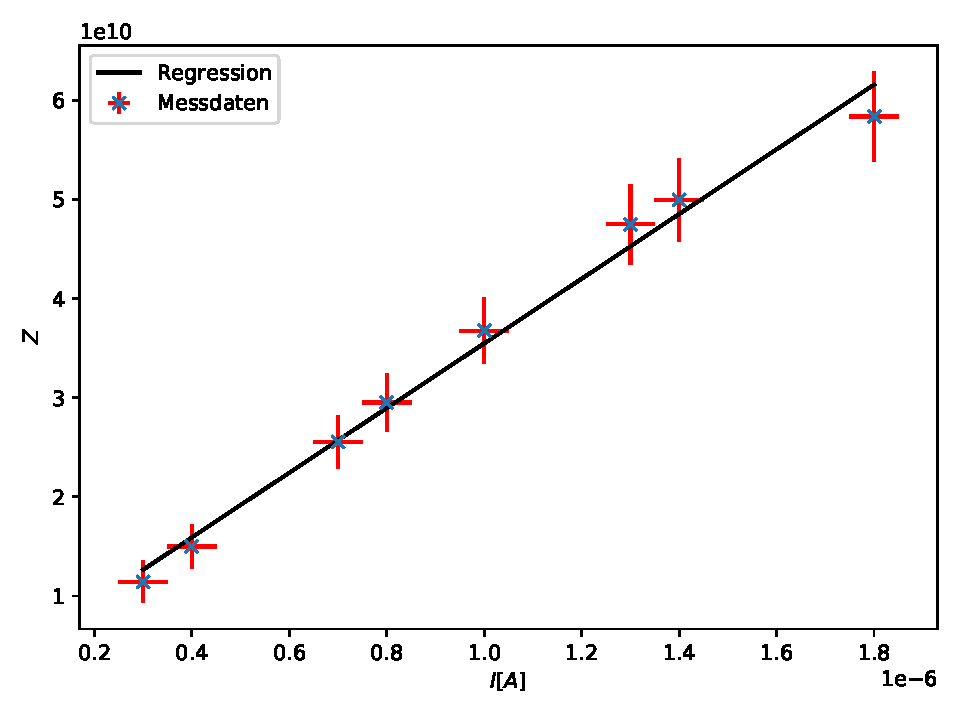
\includegraphics{auswertung/plot2.pdf}
    \caption{Anzahl an freigesetzten Ladungen pro Teilchen in Abhängigkeit der Stromstärke}
    \label{fig:Z}
\end{figure}
\noindent Die Regressionsgerade ist dabei der Form \ref{eqn:gerade}, mit den Parametern
\begin{align*}
    a &= \SI{32.6 \pm 1.39}{\peta\per\ampere}\\
    b &= \num{2.85 \pm 1.50}\si{\giga}.
\end{align*}
Die Unsicherheiten wurden dabei wieder mit \textit{nummeric python} berechnet.